\section{Results}
\label{sec:results}

\subsection{Study Selection}
\label{sec:results-selection}

The primary electronic search (Section~\ref{sec:methods-search}) returned 54 raw PubMed/MEDLINE hits on the original comparative-design question, 48 further hits from the systematic-review/meta-analysis recheck, and 10 ClinicalTrials.gov records, screened individually across four rounds (2026-07-18 to 2026-07-20). Round 3's citation-chasing pass against the largest existing phage-therapy meta-analysis's risk-of-bias table \parencite{Liu2025_ijaa} surfaced five uncatalogued records --- \textcite{Krakhotkin2025_currurol}, \textcite{Leitner2021_lancetid_pyophage}, \textcite{Karn2024_ijlew}, \textcite{Rhoads2009_jwoundcare}, and \textcite{Stanley2025_themicrobe_cyphy} --- of which only Leitner et al.\ entered the analytic dataset (extracted, excluded from pooling; Section~\ref{sec:methods-selection}); Krakhotkin et al.\ was excluded outright (zero \textit{P.\ aeruginosa} cases); Rhoads et al.\ failed eligibility on a structural ground (saline, not antibiotic, comparator); and Karn et al.\ and Stanley et al.\ remain conditionally eligible pending a full-text subgroup confirmation not completed this round, carried here as open items still to be resolved. Round 4's targeted antibiotic-only-cohort search returned 44 hits, none containing a phage arm --- confirming, not resolving, the absent monotherapy comparator. A supplementary, non-PRISMA, single-reviewer screen of a 201-document PDF corpus contributed 9 further candidates after excluding 3 duplicates; 2 of the 9 required correction on full-text review, Krakhotkin et al.\ (above) and an immunological sub-study \parencite{Dan2023_jid} confirmed to duplicate Patient 1 in \textcite{Aslam2019_ajt} -- net 8 unique new records once Krakhotkin's cross-channel duplication with the citation-chasing pass is resolved. The remaining six included studies (\textcite{Pirnay2024_natmicrobiol}, \textcite{Onallah2023_med}, \textcite{Weiner2025_natcomms}, \textcite{Jault2019_phagoburn}, the Phase 1b/2a inhaled-phage cystic-fibrosis trial \parencite{Armata_swarmpa}, and \textcite{Aslam2019_ajt}) were identified during this review's initial discovery-phase literature scoping, an earlier WebSearch/WebFetch-based pass that predates the four documented, structured-query rounds above and was not itself run with recorded, countable hits per query -- a disclosed methodological gap, not a hidden one (Figure~\ref{fig:prisma-flow}). A broad topical PubMed/MEDLINE search (481 records over the pre-specified 2016--2026 window; Section~\ref{sec:methods-search}), run to place PubMed on the same topical footing as Scopus rather than only the narrow comparative-design rounds above, recovered the eligible clinical studies already identified but added no unique-new record; a dedicated screen of its 2016--2018 sub-window found only preclinical work beyond the already-included Duplessis et al.\ (2018) and PhagoBurn. Finally, a native Scopus database search (860 records screened; 2026-07-23; Section~\ref{sec:methods-search}) --- the third core database alongside PubMed/MEDLINE and ClinicalTrials.gov --- substantially enlarged the corpus, adding ten eligible studies the earlier rounds had missed: K\"ohler et al.\ (2023), a single inhaled-phage MDR case; Chan et al.\ (2025), a nine-patient nebulized-phage cystic-fibrosis cohort split into an MDR (n=7) and a PDR (n=2) arm; and eight further human clinical \textit{P.\ aeruginosa} phage-therapy reports (Law et al.\ 2019; Hahn et al.\ 2023; Lev\^eque et al.\ 2023; Duplessis et al.\ 2018; Denis et al.\ 2026; Malhotra et al.\ 2026; Yang et al.\ 2025; Li et al.\ 2025 --- an 88-year-old woman with an MDR biliary-tract infection, previously carried as a pending record and now resolved from two concordant secondary sources). The native search also corrected one earlier provisional exclusion --- Law et al.\ (2019), previously set aside as a presumed conference abstract from the same San Diego AB-PA01 program as \textcite{Aslam2019_ajt}, is a full peer-reviewed report of a distinct MDR cystic-fibrosis patient --- and documented four exclusions: Van Nieuwenhuyse et al.\ (2022), a single XDR case already counted within \textcite{Pirnay2024_natmicrobiol}'s Belgian-consortium cohort; Zurabov et al.\ (2023), an ICU phage-monotherapy case series whose \textit{P.\ aeruginosa} outcomes cannot be separated from a multi-pathogen cohort (otherwise a rare monotherapy source); Hayakawa et al.\ (2025), a multi-pathogen feasibility study with no separable \textit{P.\ aeruginosa} outcome; and Chung et al.\ (2025), a perspective article rather than a primary study. That a native Scopus search roughly doubled the pooling-eligible corpus (from 13 to 23 studies) confirms the earlier PubMed-only coverage gap was real and material, and validates searching Scopus natively rather than through a federated adjunct. Finally, a peer-review landmark-case screen (Section~\ref{sec:methods-search}) added two further eligible studies that no keyword search had captured --- \textcite{Chan2018_omko1_emph}, the canonical OMKO1 case of an MDR aortic Dacron-graft infection (local phage plus ceftazidime, resolved without recurrence), and \textcite{Arya2026_pji_natcomms}, an MDR periprosthetic joint infection treated with phage monotherapy --- bringing the pooling-eligible corpus to 25 studies, while confirming that Rubalskii et al.\ (2020, a multi-pathogen series with no \textit{Pseudomonas}-separable outcome) and Cano et al.\ (2021, a \textit{Klebsiella} case) are correctly outside it.

The final analytic dataset contains 31 study-arms across 26 studies. One arm, \textcite{Leitner2021_lancetid_pyophage}, is excluded from all pooling as a six-pathogen, trial-wide aggregate with no \textit{Pseudomonas}-specific breakdown (Section~\ref{sec:methods-selection}), leaving \textbf{30 pooling-eligible study-arms across 25 studies}, contributing 108 patients. \Cref{fig:prisma-flow} reconciles every count above -- across all identification channels, the screening/eligibility funnel, the documented exclusions and pending records at full-text assessment, and the split between the 26 studies in the analytic dataset and the 25 pooling-eligible for quantitative synthesis -- into a single PRISMA 2020-adapted flow diagram. (\citeauthor{Pirnay2024_natmicrobiol}'s cohort contributes 3 of these 31 arms, not 1 -- see Section~\ref{sec:results-characteristics} for the resistance-stratified re-extraction that produced this split.)

\begin{figure}[htbp]
\centering
\footnotesize
\resizebox{\textwidth}{!}{
% PRISMA 2020-adapted flow diagram for this review's actual, disclosed
% multi-channel identification process (see Methods, Section 3.2 and
% Results, Section 4.1 for the narrative and every count used below;
% full explanatory detail is carried in the figure caption, not here --
% box text is deliberately terse, standard PRISMA-diagram practice).
% Bare tikzpicture content only -- wrapped by a figure/caption in results.tex.
% Core databases: PubMed/MEDLINE + ClinicalTrials.gov + Scopus (native, full
% 860-record RIS export, 2026-07-23); the native Scopus search added the nine
% clinical studies the PubMed-only rounds had missed and corrected one prior
% exclusion. Two further supplementary channels (citation-chasing; a 201-doc
% PDF/Elicit corpus) and this review's earlier discovery-phase scoping are
% shown as distinct, clearly-labelled non-core channels.
\begin{tikzpicture}[
  font=\scriptsize,
  box/.style={draw, rectangle, align=left, text width=2.7cm, inner sep=2.5pt, rounded corners=1pt, minimum height=2.3cm},
  wide/.style={draw, rectangle, align=left, text width=14.4cm, inner sep=4pt, rounded corners=1pt},
  lbl/.style={font=\scriptsize\bfseries},
  arr/.style={-{Latex[length=2mm]}, thick}
]

% ============ Row Y-coordinates ============
% Row 1 identification (y=0)   Row 2 screening (y=-3.2)
% Row 3 eligibility (y=-6.3)   Row 4 excluded/pending/included (y=-9.1)
% Row 5 quantitative synthesis (y=-13.0)

% --- Row 1: Identification (5 channels), x = 0, 3.0, 6.0, 9.0, 12.0 ---
\node[box] (db)    at (0,0)    {\textbf{PubMed/MEDLINE + ClinicalTrials.gov}\\topical search $n=481$ (2016--2026)\\$+$ 4 targeted comparative rounds (146)\\$+$ CT.gov (10)};
\node[box] (scop)  at (3.0,0)  {\textbf{Scopus (native)}\\full RIS export, TITLE-ABS-KEY, PUBYEAR${>}$2018\\$n=860$ records};
\node[box] (cite)  at (6.0,0)  {\textbf{Citation-chasing}\\of a prior meta-analysis's RoB table \parencite{Liu2025_ijaa}\\$n=5$};
\node[box] (pdf)   at (9.0,0)  {\textbf{Supplementary corpus}\\201-doc.\ PDF/Elicit screen (non-PRISMA)\\$n=201$};
\node[box] (disc)  at (12.0,0) {\textbf{Discovery-phase scoping}\\earlier WebSearch/WebFetch pass\\$n=6$};
\node[lbl, above=1mm of db.north west, anchor=south west] {IDENTIFICATION};

% --- Row 2: Screening outcomes per channel, y = -3.2 ---
\node[box] (db-out)   at (0,-3.2)   {481 topical records screened; eligible clinical studies all PubMed-indexed and \textbf{already captured via Scopus} (0 unique-new; 2016--2018 sub-window all preclinical); the 4 comparative rounds found no dual-arm study};
\node[box] (scop-out) at (3.0,-3.2) {860 screened on type/title $\rightarrow$ 28 clinical candidates $\rightarrow$ \textbf{10 studies added} (K\"ohler, Chan $+$ 8 new), 3 excluded; rest already held};
\node[box] (cite-out) at (6.0,-3.2) {5 proceed to full-text eligibility};
\node[box] (pdf-out)  at (9.0,-3.2) {189 excluded, 12 pass rubric $-$3 dupes $-$1 (Krakhotkin) $\rightarrow$ \textbf{8 proceed}};
\node[box] (disc-out) at (12.0,-3.2){6 proceed to full-text eligibility};
\node[lbl] at (-2.4,-3.2) {SCREENING};

% --- Row 3: Eligibility summary, y = -6.3 ---
\node[wide] (elig) at (6.0,-6.3) {\textbf{Assessed for full-text eligibility: $n=39$ unique records} (5 citation-chased $+$ 8 via the PDF corpus $+$ 6 via discovery-phase scoping $+$ 9 new via the native Scopus search $+$ 5 held records re-confirmed $+$ 4 landmark cases flagged at peer review $+$ 2 further records named at peer review, round 2)};
\node[lbl] at (-2.4,-6.3) {ELIGIBILITY};

% --- Row 4: Excluded / Pending / Included, y = -9.1 ---
\node[box, text width=4.6cm, minimum height=4.6cm] (excl) at (0.6,-9.1) {\textbf{Excluded, $n=9$}\\$\bullet$ Krakhotkin 2025 -- wrong pathogen\\$\bullet$ Cano 2021 -- wrong pathogen (\textit{Klebsiella})\\$\bullet$ Rhoads 2009 -- no antibiotic comparator\\$\bullet$ Dan 2023 -- duplicate (Aslam)\\$\bullet$ Van Nieuwenhuyse 2022 -- duplicate (Pirnay consortium)\\$\bullet$ Zurabov 2023, Rubalskii 2020 -- multi-pathogen, not separable\\$\bullet$ Hayakawa 2025 -- multi-pathogen feasibility\\$\bullet$ Chung 2025 -- review/perspective};
\node[box, text width=4.6cm, minimum height=4.6cm] (pend) at (6.0,-9.1) {\textbf{Reports not retrieved, $n=1$}\\$\bullet$ Maddocks 2019 -- eligible in principle; no abstract indexed, full text not retrieved, no outcome extractable\\\smallskip \textbf{Pending / unresolved, $n=2$}\\$\bullet$ Karn 2024\\$\bullet$ Stanley 2025 (CYPHY)\\Conditionally eligible; outstanding, not dropped};
\node[box, text width=4.6cm, minimum height=4.6cm] (incl) at (11.4,-9.1) {\textbf{Included, $n=27$ studies}\\(32 study-arms)\\\smallskip Ten added by the native Scopus search (incl.\ K\"ohler 2023, Chan 2025, Law 2019, Li 2025); 2 landmark cases flagged at peer review (Chan 2018, Arya 2026); 1 added at peer review round 2 (Ferry 2021)};
\node[lbl] at (-2.4,-9.1) {};

% --- Row 5: Quantitative synthesis, y = -13.0 ---
\node[wide] (synth) at (6.0,-13.0) {\textbf{Included in quantitative synthesis (pooling): $n=26$ studies, 30 study-arms.} 2 arms retained in the analytic dataset but excluded from all pooling: Leitner et al.\ 2021 (reported only as a six-pathogen, trial-wide aggregate with no \textit{Pseudomonas}-specific breakdown), and Liu et al.\ 2025 Patient 1 (antibiogram shows non-susceptibility to one agent only, below the MDR population criterion; the series' PDR patient is retained).};
\node[lbl] at (-2.4,-13.0) {INCLUDED};

% ============ Arrows ============
\draw[arr] (db.south) -- (db-out.north);
\draw[arr] (scop.south) -- (scop-out.north);
\draw[arr] (cite.south) -- (cite-out.north);
\draw[arr] (pdf.south) -- (pdf-out.north);
\draw[arr] (disc.south) -- (disc-out.north);

\draw[arr] (db-out.south) |- ++(0,-0.9) -| (elig.north -| db.center);
\draw[arr] (scop-out.south) |- ++(0,-0.9) -| (elig.north -| scop.center);
\draw[arr] (cite-out.south) -- (elig.north -| cite.center);
\draw[arr] (pdf-out.south) |- ++(0,-0.9) -| (elig.north -| pdf.center);
\draw[arr] (disc-out.south) |- ++(0,-0.9) -| (elig.north -| disc.center);

\draw[arr] (elig.south -| excl.center) -- (excl.north);
\draw[arr] (elig.south) -- (pend.north);
\draw[arr] (elig.south -| incl.center) -- (incl.north);

\draw[arr] (incl.south) |- ++(0,-1.2) -| (synth.north -| incl.center);

\end{tikzpicture}

}
\caption{PRISMA 2020-adapted flow diagram of study identification and selection. This review's identification process departed from a single linear database search: multiple channels contributed candidate records -- a structured, documented PubMed/MEDLINE and ClinicalTrials.gov search across four rounds (Section~\ref{sec:methods-search}), a native Scopus database search (860 records, 2026-07-23) that added ten eligible studies (K\"ohler et al., 2023; Chan et al., 2025; and Law et al., 2019, Hahn et al., 2023, Lev\^eque et al., 2023, Duplessis et al., 2018, Denis et al., 2026, Malhotra et al., 2026, Yang et al., 2025, and Li et al., 2025), corrected the earlier provisional exclusion of Law et al.\ (2019), and documented exclusions (Van Nieuwenhuyse et al., 2022; Zurabov et al., 2023; Hayakawa et al., 2025; Chung et al., 2025), citation-chasing of a prior meta-analysis's risk-of-bias table \parencite{Liu2025_ijaa}, a supplementary single-reviewer screen of a 201-document PDF/Elicit corpus (a non-PRISMA source, explicitly flagged as such in Section~\ref{sec:methods-search}), this review's earlier, less formally documented discovery-phase literature scoping, and a peer-review landmark-case screen that added two further eligible studies (Chan et al., 2018 [OMKO1]; Arya et al., 2026) and confirmed two more exclusions (Rubalskii et al., 2020, multi-pathogen; Cano et al., 2021, \textit{Klebsiella}). One record (Krakhotkin et al., 2025) was independently surfaced by two channels and is counted once, at the point its cross-channel duplication was recognized during full-text eligibility review. Two records (Karn et al., 2024; Stanley et al., 2025) remain conditionally eligible pending a full-text \textit{Pseudomonas}-subgroup confirmation not completed this round and are reported as outstanding rather than folded into either the included or excluded counts. All counts are traceable to Sections~\ref{sec:methods-search} and \ref{sec:results-selection} and to \texttt{data/cleaned/phage\_therapy\_extraction\_dataset.csv}. Source: this review's own search and screening records; see the claim-source map for the per-count traceability audit.}
\label{fig:prisma-flow}
\end{figure}

\subsection{Study Characteristics}
\label{sec:results-characteristics}

The 30 pooling-eligible arms span publication years 2018--2026 and multiple countries or multicentre consortia. Design is predominantly single-patient: 17 case-report studies contributing 18 arms (\textcite{Tkhilaishvili2020_aac}, \textcite{Blasco2023_frontmed}, \textcite{Ferry2022_natcomms}, \textcite{Ngauy2026_asmcr}, \textcite{Racenis2022_frontmed}, \textcite{Racenis2023_viruses}, \citeauthor{Aslam2019_ajt}'s \citeyear{Aslam2019_ajt} two lung-transplant patients, K\"ohler et al.'s (2023) single inhaled-phage case, the seven single-patient reports added by the native Scopus search --- Law et al.\ 2019, Lev\^eque et al.\ 2023, Duplessis et al.\ 2018, Denis et al.\ 2026, Malhotra et al.\ 2026, Yang et al.\ 2025, and Li et al.\ 2025 --- and the two single-patient landmark cases added through the peer-review landmark-case screen, \textcite{Chan2018_omko1_emph} and \textcite{Arya2026_pji_natcomms}), 4 case series contributing 6 arms (\citeauthor{Liu2025_mlife_perinephric}'s \citeyear{Liu2025_mlife_perinephric} two-patient perinephric-abscess series, \citeauthor{Onallah2023_med}'s \citeyear{Onallah2023_med} PASA16 series, Chan et al.'s (2025) nine-patient cystic-fibrosis cohort split into an MDR and a PDR arm, and Hahn et al.'s (2023) two-patient cystic-fibrosis series), 3 randomized trials (each contributing only its phage arm, since no arm met this review's monotherapy definition), and 1 retrospective cohort contributing 3 resistance-stratified arms (\citeauthor{Pirnay2024_natmicrobiol} \citeyear{Pirnay2024_natmicrobiol}). Arm size ranges from single patients (20 of 30 arms) to 23 (Pirnay's MDR-stratified arm), 15 (the Onallah PASA16 series), and the 9-patient Chan cystic-fibrosis cohort (split 7 MDR + 2 PDR); the 10 arms with more than one patient together account for 88 of the corpus's 108 patients.

\citeauthor{Pirnay2024_natmicrobiol}'s cohort was re-extracted in full for this review (Section~\ref{sec:methods-extraction}): the paper's open-access supplementary tables (PMC11153159) report per-patient outcomes for all 100 consecutive cases, of which 49 targeted \textit{P.\ aeruginosa} specifically -- matching the paper's own stated figure exactly. Of those 49, 17 are classified ``usual drug resistance'' in the source data and therefore do \emph{not} meet this review's MDR/XDR/PDR eligibility criterion; they are excluded. The remaining 32 patients split into three resistance-stratified arms: 7 XDR, 23 MDR, and 2 PDR. This supersedes an earlier 11-patient subset drawn only from the paper's main-text case narratives; cross-validation against that subset found exact agreement on 9 of 11 patients; the other 2 (case \#30 and \#71) are usual-drug-resistance rather than MDR/XDR/PDR and are now excluded. This is a genuine eligibility correction, made possible only once per-patient resistance data became available -- new information, not an error in the original 11-patient read.

Resistance classification (Section~\ref{sec:methods-extraction}) assigns 17 arms MDR, 4 XDR, 4 PDR, and 5 not-classifiable; four MDR calls and three of the four XDR calls were independently re-derived from a reported antibiogram, the remainder resting on the primary study's own label (including all three of Pirnay's new resistance-stratified arms, which rest on that paper's own per-patient antibiogram-based classification, not an independent re-derivation by this review team -- see the classification-sensitivity check, Section~\ref{sec:results-robustness}). Route (collapsed) splits 10 other (multi-route), 7 inhaled/nebulized, 5 intravenous, 6 topical/local, and 2 of unspecified route (Malhotra et al.\ 2026 and Arya et al.\ 2026, route not reported in the available source). Modality is overwhelmingly combination therapy (28 of 30 arms); the two remaining arms are phage monotherapy --- \textcite{Jault2019_phagoburn} against a standard-wound-care comparator and \textcite{Arya2026_pji_natcomms}, an intermittent phage-only regimen with no antibiotic --- so the phage-monotherapy stratum now holds two arms, while no arm is coded pure antibiotic monotherapy. \Cref{tab:study-characteristics} tabulates all 31 study-arms across 26 studies at the arm level, including the one arm excluded from pooling.

\begin{table}[htbp]
\centering
\scriptsize
\setlength{\tabcolsep}{3.5pt}
\begin{threeparttable}
\caption{Study characteristics, all 31 extracted study-arms}
\label{tab:study-characteristics}
\begin{tabular}{llccccll}
\toprule
Study & Country/region & Design & $n$ & Resistance & Route & Modality & Pooling \\
\midrule
Tkhilaishvili 2020 & Germany & Case rpt. & 1 & XDR & Topical & Combo & Pooled \\
Blasco 2023 & Spain & Case rpt. & 1 & MDR & IV & Combo & Pooled \\
Ngauy 2026 & USA & Case rpt. & 1 & XDR & IV & Combo & Pooled \\
Ferry 2022 & France & Case rpt. & 1 & PDR & Other & Combo & Excluded$^{a}$ \\
Liu 2025 & China & Case series & 1 & NC & Topical & Combo & Excluded$^{a}$ \\
Liu 2025 & China & Case series & 1 & PDR & Topical & Combo & Pooled \\
Racenis 2023 & Latvia & Case rpt. & 1 & MDR & Other & Combo & Excluded$^{a}$ \\
Racenis 2022 & Latvia & Case rpt. & 1 & MDR & Topical & Combo & Pooled \\
Onallah 2023 & Israel & Case series & 15 & NC & Other & Combo & Pooled \\
Weiner 2025 & Multi. & RCT & 7 & NC & Inhaled & Combo & Excluded$^{a}$ \\
Jault 2019 & Multi.\ (EU) & RCT & 13 & NC & Topical & Phage mono & Excluded$^{a}$ \\
Leitner 2021 & Georgia & RCT & 28 & NC & Other & Phage mono & Excluded$^{a}$ \\
SWARM-P.a.\ 2022 & Multi.\ (CF) & RCT & 10 & NC & Inhaled & Combo & Excluded$^{a}$ \\
Aslam 2019 & USA & Case rpt. & 1 & MDR & Other & Combo & Pooled \\
Aslam 2019 & USA & Case rpt. & 1 & MDR & IV & Combo & Pooled \\
Pirnay 2024 & Belgium & Retro. & 7 & XDR & Other & Combo & Pooled \\
Pirnay 2024 & Belgium & Retro. & 23 & MDR & Other & Combo & Pooled \\
Pirnay 2024 & Belgium & Retro. & 2 & PDR & Other & Combo & Pooled \\
K\"ohler 2023 & Switzerland & Case rpt. & 1 & MDR & Inhaled & Combo & Pooled \\
Chan 2025 & USA & Case series & 7 & MDR & Inhaled & Combo & Pooled \\
Chan 2025 & USA & Case series & 2 & PDR & Inhaled & Combo & Pooled \\
Law 2019 & USA & Case rpt. & 1 & MDR & IV & Combo & Pooled \\
Hahn 2023 & USA & Case series & 2 & MDR & Inhaled & Combo & Pooled \\
Lev\^eque 2023 & France & Case rpt. & 1 & XDR & Other & Combo & Pooled \\
Duplessis 2018 & USA & Case rpt. & 1 & MDR & IV & Combo & Pooled \\
Denis 2026 & France & Case rpt. & 1 & MDR & Other & Combo & Pooled \\
Malhotra 2026 & USA & Case rpt. & 1 & MDR & NR & Combo & Pooled \\
Yang 2025 & China & Case rpt. & 1 & MDR & Inhaled & Combo & Pooled \\
Li 2025 & China & Case rpt. & 1 & MDR & Other & Combo & Pooled \\
Chan 2018 & USA & Case rpt. & 1 & MDR & Topical & Combo & Pooled \\
Arya 2026 & USA & Case rpt. & 1 & MDR & NR & Phage mono & Pooled \\
Ferry 2021 & France & Case rpt. & 1 & NC & Topical & Combo & Pooled \\
Maddocks 2019 & Australia & Case rpt. & 1 & NC & Other & Combo & Pooled \\
Aslam 2020 & United States & Case series & 1 & MDR & IV & Combo & Pooled \\
Aslam 2020 & United States & Case series & 1 & NC & IV & Combo & Pooled \\
Aslam 2020 & United States & Case series & 1 & NC & IV & Combo & Pooled \\
Cesta 2023 & Italy & Case rpt. & 1 & NC & Topical & Combo & Pooled \\
Khatami 2021 & Australia & Case rpt. & 1 & NC & NR & Combo & Pooled \\
Zaldastanishvili 2021 & Georgia & Case series & 1 & NC & Other & Phage mono & Pooled \\
Zaldastanishvili 2021 & Georgia & Case series & 1 & NC & Other & Phage mono & Pooled \\
Green 2023 & USA & Case series & 1 & NC & Other & Combo & Pooled \\
Casazza 2025 & USA & Case rpt. & 1 & MDR & Other & Combo & Pooled \\
Teney 2024 & France & Case rpt. & 1 & XDR & Other & Combo & Pooled \\
Li 2023 & China & Case rpt. & 1 & MDR & Inhaled & Combo & Pooled \\
Chen 2022 & China & Case rpt. & 1 & NC & NR & Combo & Pooled \\
Jennes 2017 & Belgium & Case rpt. & 1 & XDR & Other & Phage mono & Excluded$^{a}$ \\
Chung 2026 & Singapore & Case rpt. & 1 & $<$MDR & IV & Combo & Excluded$^{a}$ \\
Ronit 2024 & Denmark & Case rpt. & 1 & $<$MDR & IV & Combo & Excluded$^{a}$ \\
Rubalskii 2020 & Germany & Case series & 1 & NC & Topical & Combo & Pooled \\
Pardo-Freire 2025 & Spain & Case rpt. & 1 & MDR & Inhaled & Combo & Pooled \\
\bottomrule
\end{tabular}

\begin{tablenotes}\footnotesize
\item \textit{Notes:} One row per study-arm (the unit of extraction; Section~\ref{sec:methods-extraction}), not per study -- \textcite{Liu2025_mlife_perinephric}, \citeauthor{Aslam2019_ajt} (\citeyear{Aslam2019_ajt}), and Chan et al.\ (2025) each contribute 2 arms. $n$ is the arm-level patient count. Resistance: MDR/XDR/PDR per \textcite{Magiorakos2012_mdrxdr} where independently re-derivable from a reported antibiogram, else the primary study's own label; NC = not-classifiable. Route and Modality are collapsed to their controlled category (parenthetical qualifiers, e.g.\ specific multi-route detail, are stripped; see \texttt{data/cleaned/phage\_therapy\_extraction\_dataset.csv} and its codebook for the uncollapsed text). Pooling reflects this review's pre-specified pooling-eligibility rule (Section~\ref{sec:methods-selection}), not risk of bias or study quality.
\item[a] \textcite{Leitner2021_lancetid_pyophage} is retained in the analytic dataset but excluded from all pooling: its outcomes are reported only as a six-pathogen, trial-wide aggregate with no \textit{Pseudomonas}-specific breakdown (Section~\ref{sec:methods-selection}).
\item Source: \texttt{scripts/R/09\_table1\_characteristics.R}, reading \texttt{data/cleaned/phage\_therapy\_extraction\_dataset.csv}.
\end{tablenotes}
\end{threeparttable}
\end{table}

\subsection{Risk of Bias}
\label{sec:results-rob}

Risk-of-bias ratings (ROBINS-I, RoB2, the JBI case-series tool, and \textcite{Murad2018_casereports} for reports of one to three patients; Section~\ref{sec:methods-rob}) are now complete for all 31 study-arms, closing a gap disclosed as outstanding earlier in this review. The 4 randomized trials rate: PhagoBurn \parencite{Jault2019_phagoburn} High risk (unmasked clinicians, stopped early for insufficient efficacy); \citeauthor{Leitner2021_lancetid_pyophage} \citeyear{Leitner2021_lancetid_pyophage} and \citeauthor{Weiner2025_natcomms} \citeyear{Weiner2025_natcomms} Some concerns (a partially open-label comparator arm and moderate attrition for the former, a small and incompletely-reported safety population for the latter); the SWARM-P.a./AP-PA02 trial \parencite{Armata_swarmpa} Low risk, confirmed from ClinicalTrials.gov's structured results directly. On the JBI checklist, \citeauthor{Pirnay2024_natmicrobiol}'s cohort rates Low risk (explicitly consecutive, complete, fully transparent per-patient reporting this review team examined firsthand), the \citeauthor{Onallah2023_med} PASA16 series rates Low-to-moderate risk (two Unclear items reflecting abstract-only access), and Chan et al.'s (2025) two-arm cystic-fibrosis series likewise rates Low-to-moderate risk. K\"ohler et al.'s (2023) single inhaled-phage case, rated under the Murad et al.\ tool, rates Low-to-moderate risk. The eight studies added by the native Scopus search likewise rate Low-to-moderate risk (seven single-patient case reports under the Murad et al.\ tool; Hahn et al.'s (2023) two-patient series under the JBI checklist), as do the two single-patient landmark cases added during peer review (\textcite{Chan2018_omko1_emph} and \textcite{Arya2026_pji_natcomms}, both under the Murad et al.\ tool). Full per-domain judgments and rationale are in \texttt{quality\_reports/risk\_of\_bias\_assessment\_phage\_therapy\_mdr\_pseudomonas.md}; a per-domain tabulation of the single-patient case reports' ratings was not separately retained, a disclosed, low-consequence gap given these are the simplest, lowest-failure-mode cases for the Murad et al.\ tool. These ratings feed the GRADE certainty assessment reported in Section~\ref{sec:results-grade}.

\subsection{Synthesis of Pooled Outcomes}
\label{sec:results-synthesis}

Of 37 outcome-stratum cells defined by the pre-specified three-way stratification, 15 met the threshold of at least 3 independent studies and 20 patients (\Cref{tab:pooled-estimates}); the remaining 22 are narrated in \Cref{tab:not-pooled}. Pooled clinical success across all 20 contributing studies (67 patients) was 77.6\% (95\% CI 65.4--86.4\%; $\tau^2=0$, 95\% prediction interval 65.4--86.4\%; \Cref{fig:forest-success-overall}), directionally consistent with prior non-stratified syntheses \parencite{ElHaddad2019_eskape,Uyttebroek2022_lancetid,Liu2025_ijaa} --- explicitly secondary and contextual regardless, since the underlying population is compassionate-use and selected for refractory infection, not a treatment effect. Pooled eradication across 19 studies (60 patients) was 55.1\% (95\% CI 29.4--78.4\%), and pooled mortality across 23 studies (86 patients) was 10.5\% (95\% CI 5.4--19.4\%). The eradication estimate carries a wide interval ($\tau^2=2.11$) that reflects genuine heterogeneity by infection setting: several chronic lung infections in the corpus --- including a Kartagener-syndrome case (K\"ohler et al., 2023) and a nine-patient cystic-fibrosis cohort (Chan et al., 2025) --- reduced sputum bacterial load without eradicating the organism, whereas acute infections at other sites were more often cleared, so the pooled proportion spans a range from chronic respiratory colonisation (rarely cleared even when patients improve clinically) to complete eradication. We read this wide interval as a genuine feature of the clinical spectrum, not as noise.

\begin{table}[htbp]
\centering
\scriptsize
\setlength{\tabcolsep}{3pt}
\begin{threeparttable}
\caption{Pooled outcome-stratum cells meeting the pre-specified pooling threshold}
\label{tab:pooled-estimates}
\begin{tabular}{lcccccccc}
\toprule
Outcome -- Stratum & $k$ & Arms & $N$ & Pooled proportion [95\% CI] & $\tau^2$ & 95\% prediction interval & Model \\
\midrule
Clinical success -- Overall & 21 & 24 & 67 & 77.6\% [65.4\%, 86.4\%] & 0.000 & [65.4\%, 86.4\%] & GLMM \\
Safety (>=1 AE) -- Overall & 17 & 20 & 50 & 16.0\% [7.8\%, 29.9\%] & 0.000 & [7.8\%, 29.9\%] & GLMM \\
Eradication -- Overall & 19 & 23 & 59 & 52.9\% [27.8\%, 76.6\%] & 2.045 & [4.6\%, 96.3\%] & GLMM \\
Mortality -- Overall & 22 & 26 & 63 & 12.7\% [6.3\%, 24.1\%] & 0.000 & [6.3\%, 24.1\%] & GLMM \\
Clinical success -- Resistance: MDR & 14 & 15 & 37 & 75.7\% [57.8\%, 87.6\%] & 0.000 & [57.8\%, 87.6\%] & GLMM \\
Safety (>=1 AE) -- Resistance: MDR & 12 & 13 & 36 & 16.7\% [7.0\%, 34.6\%] & 0.000 & [7.0\%, 34.6\%] & GLMM \\
Eradication -- Resistance: MDR & 14 & 15 & 43 & 58.1\% [12.5\%, 93.1\%] & 7.152 & [0.3\%, 99.8\%] & GLMM$^\ddagger$ \\
Mortality -- Resistance: MDR & 16 & 17 & 46 & 6.5\% [1.9\%, 19.8\%] & 0.000 & [1.9\%, 19.8\%] & GLMM \\
Clinical success -- Route: other & 8 & 10 & 53 & 77.4\% [61.9\%, 87.8\%] & 0.000 & [61.9\%, 87.8\%] & GLMM \\
Safety (>=1 AE) -- Route: other & 7 & 9 & 38 & 15.8\% [6.3\%, 34.3\%] & 0.000 & [6.3\%, 34.3\%] & GLMM \\
Eradication -- Route: other & 7 & 9 & 38 & 63.2\% [44.1\%, 78.8\%] & 0.000 & [44.1\%, 78.8\%] & GLMM \\
Mortality -- Route: other & 7 & 9 & 38 & 16.0\% [3.6\%, 48.9\%] & 0.030 & [3.5\%, 50.1\%] & GLMM \\
\bottomrule
\end{tabular}

\begin{tablenotes}
\small
\item \textit{Notes:} Sample: 30 pooling-eligible study-arms across 25 studies, 108 patients (\texttt{data/cleaned/phage\_therapy\_extraction\_dataset.csv}). NC = not-classifiable. A cell is reported here only if it contains at least 3 independent studies and at least 20 pooled patients; all other cells appear in \Cref{tab:not-pooled}. Pooled proportion, $\tau^2$, and the 95\% prediction interval are from a random-effects binomial-normal GLMM (logit link), with 95\% CIs adjusted per Hartung-Knapp-Sidik-Jonkman. Between-study heterogeneity is summarized by $\tau^2$ and the 95\% prediction interval, which for a binomial-normal GLMM are more reliable indices for proportion meta-analyses than the conventional inconsistency statistic. "Overall" rows are secondary/contextual and are not this review's primary estimand. Source: \texttt{scripts/R/04\_estimation.R}, \texttt{08\_tables.R}.
\end{tablenotes}
\end{threeparttable}
\end{table}

Four stratified categories reached the threshold for at least one outcome. The clearest is a genuine resistance class rather than a residual grab-bag: the \textbf{MDR resistance stratum is now pooled across all four outcomes} --- clinical success 75.7\% (95\% CI 57.8--87.6\%; 14 studies, 37 patients; \Cref{fig:forest-success-mdr}), safety 16.7\% (95\% CI 7.0--34.6\%; 12 studies, 36 patients), eradication 58.1\% (95\% CI 12.5--93.1\%; 14 studies, 43 patients), and mortality 6.5\% (95\% CI 1.9--19.8\%; 16 studies, 46 patients). This answers part of this review's originally-blocked core stratification aim---an MDR-specific pooled estimate now exists---but only as a fragile, single-cohort signal: \citeauthor{Pirnay2024_natmicrobiol} still supplies roughly three-fifths of the MDR clinical-success patients, and the estimate clears the threshold only under author-reported resistance labels, collapsing to three studies and four patients when classification is restricted to independently verified cases (Section~\ref{sec:results-robustness}). It does not, however, complete the aim as designed --- \textbf{XDR (4 studies, 10 patients) and PDR (3--4 studies, 4--6 patients) remain below the 20-patient threshold for every outcome} and are reported in \Cref{tab:not-pooled} as insufficient evidence, so the MDR-\emph{versus}-XDR comparison itself still cannot be made, even though MDR alone can now be estimated. The residual not-classifiable resistance bucket also reaches threshold for two outcomes: safety (4 studies, 31 patients, 21.5\%, 95\% CI 2.4--75.2\%) and mortality (3 studies, 24 patients, 4.2\%, 95\% CI 0.1--77.9\%) --- both, given the extremely wide CIs, better read as confirming these events are rare-to-uncommon in this bucket than as precise point estimates. The multi-route or otherwise unclassifiable ("other") route category is also pooled across all four outcomes (7--8 studies depending on outcome, 38--53 patients): clinical success 77.4\% (95\% CI 61.9--87.8\%), safety 15.8\% (95\% CI 6.3--34.3\%), eradication 63.2\% (95\% CI 44.1--78.8\%), mortality 16.0\% (95\% CI 3.6--48.9\%). Among the specific single routes, the inhaled/nebulized route --- enlarged as the search expanded --- now reaches the pooling threshold for one outcome: safety (5 studies, 21 patients, 30.3\%, 95\% CI 3.9--82.2\%). This safety estimate carries a very wide interval and should be read as imprecise. The corresponding inhaled/nebulized mortality cell (0 deaths across 23 patients) meets the count threshold but is a zero-event cell that is uninformative as a pooled proportion---a pooled 0.0\% with a confidence interval spanning the whole 0--100\% range conveys nothing---so it is demoted to the narrative record (\Cref{tab:not-pooled}) and reported instead by its exact one-sided rule-of-three bound: 0 of 23 deaths, upper 97.5\% one-sided bound approximately 13\%. Topical/local and intravenous still fall below threshold for every outcome. Modality stratification could not be attempted at all, since zero of the 30 arms are antibiotic monotherapy (\Cref{tab:not-pooled}, final row), consistent with Section~\ref{sec:results-selection}; the two phage-monotherapy arms (\citeauthor{Jault2019_phagoburn}'s PhagoBurn phage arm and \citeauthor{Arya2026_pji_natcomms}'s antibiotic-free periprosthetic-joint case) remain too few to form a poolable modality stratum of their own. Within the MDR stratum, one study (\citeauthor{Pirnay2024_natmicrobiol} \citeyear{Pirnay2024_natmicrobiol}) still contributes the plurality of patients --- 23 of the 37 in the MDR clinical-success pool (62\%) and a smaller 53\% of the larger 43-patient MDR eradication pool --- but the seven MDR arms added since the earlier rounds only partly dilute, and do not remove, the single-source dependence that earlier versions of this stratum carried; Section~\ref{sec:results-robustness} reports what happens to the MDR safety and mortality estimates when that one study is removed, and shows the whole MDR stratum collapsing to three studies and four patients once resistance labels are restricted to independently verified cases.

\begin{table}[htbp]
\centering
\scriptsize
\setlength{\tabcolsep}{4pt}
\begin{threeparttable}
\caption{Outcome-stratum cells reported narratively: insufficient evidence to support formal pooling}
\label{tab:not-pooled}
\begin{tabular}{lcccl}
\toprule
Outcome -- Stratum & $k$ & Arms & $N$ & Reason not pooled \\
\midrule
Clinical success -- Resistance: PDR & 2 & 2 & 3 & $k<3$, $N<20$ \\
Clinical success -- Resistance: XDR & 5 & 5 & 11 & $N<20$ \\
Safety (>=1 AE) -- Resistance: NC & 6 & 8 & 8 & $N<20$ \\
Safety (>=1 AE) -- Resistance: PDR & 2 & 2 & 3 & $k<3$, $N<20$ \\
Safety (>=1 AE) -- Resistance: XDR & 5 & 5 & 11 & $N<20$ \\
Eradication -- Resistance: NC & 6 & 7 & 7 & $N<20$ \\
Eradication -- Resistance: PDR & 3 & 3 & 5 & $N<20$ \\
Eradication -- Resistance: XDR & 5 & 5 & 11 & $N<20$ \\
Mortality -- Resistance: NC & 9 & 11 & 11 & $N<20$ \\
Mortality -- Resistance: PDR & 3 & 3 & 5 & $N<20$ \\
Mortality -- Resistance: XDR & 5 & 5 & 11 & $N<20$ \\
Clinical success -- DTR: positive & 4 & 4 & 5 & $N<20$ \\
Clinical success -- DTR: negative & 1 & 1 & 1 & $k<3$, $N<20$ \\
Clinical success -- DTR: not derivable & 28 & 32 & 74 & partial antibiogram \\
Safety (>=1 AE) -- DTR: positive & 4 & 4 & 5 & $N<20$ \\
Safety (>=1 AE) -- DTR: negative & 1 & 1 & 1 & $k<3$, $N<20$ \\
Safety (>=1 AE) -- DTR: not derivable & 21 & 25 & 54 & partial antibiogram \\
Eradication -- DTR: positive & 5 & 5 & 7 & $N<20$ \\
Eradication -- DTR: negative & 1 & 1 & 1 & $k<3$, $N<20$ \\
Eradication -- DTR: not derivable & 24 & 26 & 60 & partial antibiogram \\
Mortality -- DTR: positive & 5 & 5 & 7 & $N<20$ \\
Mortality -- DTR: negative & 1 & 1 & 1 & $k<3$, $N<20$ \\
Mortality -- DTR: not derivable & 29 & 33 & 68 & partial antibiogram \\
Clinical success -- Route: inhaled/nebulized & 4 & 4 & 4 & $N<20$ \\
Clinical success -- Route: IV & 6 & 8 & 8 & $N<20$ \\
Clinical success -- Route: topical/local & 7 & 7 & 7 & $N<20$ \\
Safety (>=1 AE) -- Route: inhaled/nebulized & 5 & 5 & 6 & $N<20$ \\
Safety (>=1 AE) -- Route: IV & 5 & 7 & 7 & $N<20$ \\
Safety (>=1 AE) -- Route: topical/local & 5 & 5 & 5 & $N<20$ \\
Eradication -- Route: inhaled/nebulized & 5 & 6 & 13 & $N<20$ \\
Eradication -- Route: IV & 5 & 5 & 5 & $N<20$ \\
Eradication -- Route: topical/local & 6 & 6 & 6 & $N<20$ \\
Mortality -- Route: inhaled/nebulized & 6 & 7 & 15 & $N<20$ \\
Mortality -- Route: IV & 6 & 8 & 8 & $N<20$ \\
Mortality -- Route: topical/local & 7 & 7 & 7 & $N<20$ \\
Modality: antibiotic monotherapy (all outcomes) & 0 & 0 & 0 & 0 arms (stratum empty) \\
\bottomrule
\end{tabular}

\begin{tablenotes}
\small
\item \textit{Notes:} Sample: 30 pooling-eligible study-arms across 25 studies. NC = not-classifiable. All 21 cells listed here either fall short of the pre-specified threshold ($k \geq 3$ studies, $N \geq 20$ patients) on at least one criterion or are uninformative as a pooled proportion; "Reason not pooled" states which applies for that cell ($k<3$: too few studies; $N<20$: too few patients despite enough studies; both may fail together; "0 events": a zero-event cell that meets the count threshold but yields an uninformative pooled proportion, reported narratively instead). Individual study-level proportions are tabulated in the underlying analysis but not pooled, per the pre-registered sparsity rule (Section~\ref{sec:methods-outcomes}). This includes XDR and PDR for every outcome (failing on $N$ alone -- both meet the study-count threshold), every specific single route apart from the pooled "other" category and the newly-pooled inhaled/nebulized safety cell, and the inhaled/nebulized mortality cell, which meets the count threshold but is demoted for reporting zero events (Section~\ref{sec:results-synthesis}). The final row reports the absent antibiotic-monotherapy stratum across all four outcomes. Source: \texttt{scripts/R/04\_estimation.R}, \texttt{08\_tables.R}.
\end{tablenotes}
\end{threeparttable}
\end{table}

\begin{figure}[htbp]
\centering
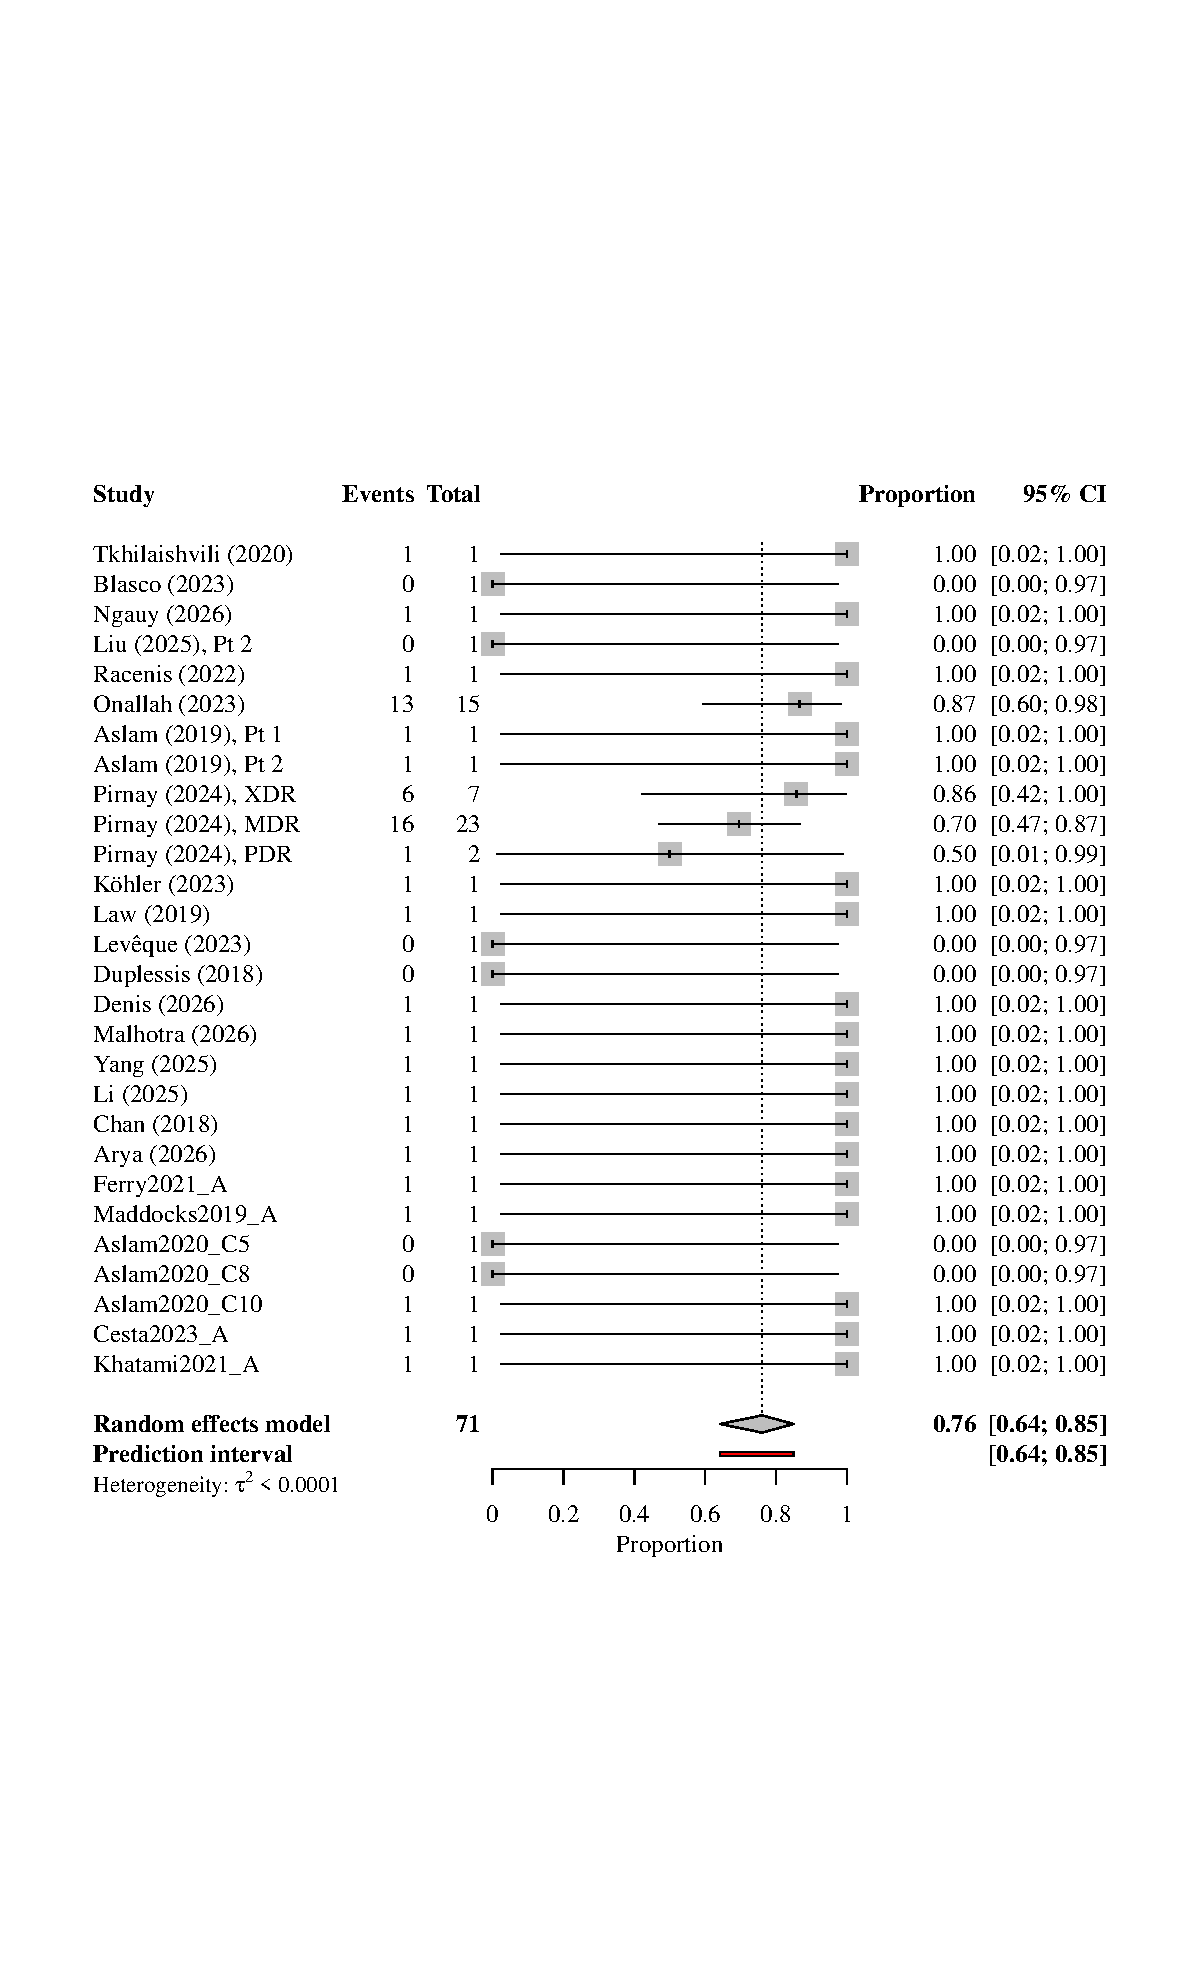
\includegraphics[width=0.8\textwidth]{figures/phage_therapy_mdr_pseudomonas/forest_clinical_success_overall.pdf}
\caption{Forest plot: pooled clinical success, overall (secondary/contextual). Each row is one of the 20 studies contributing clinical-success data (67 patients); markers show the study-specific proportion with 95\% CI, the diamond shows the GLMM pooled estimate (77.6\%, 95\% CI 65.4--86.4\%). Reported for comparability with prior non-stratified syntheses, not as this review's primary estimand. Source: \texttt{scripts/R/07\_figures.R}.}
\label{fig:forest-success-overall}
\end{figure}

\begin{figure}[htbp]
\centering
\begin{subfigure}{0.48\textwidth}
\centering
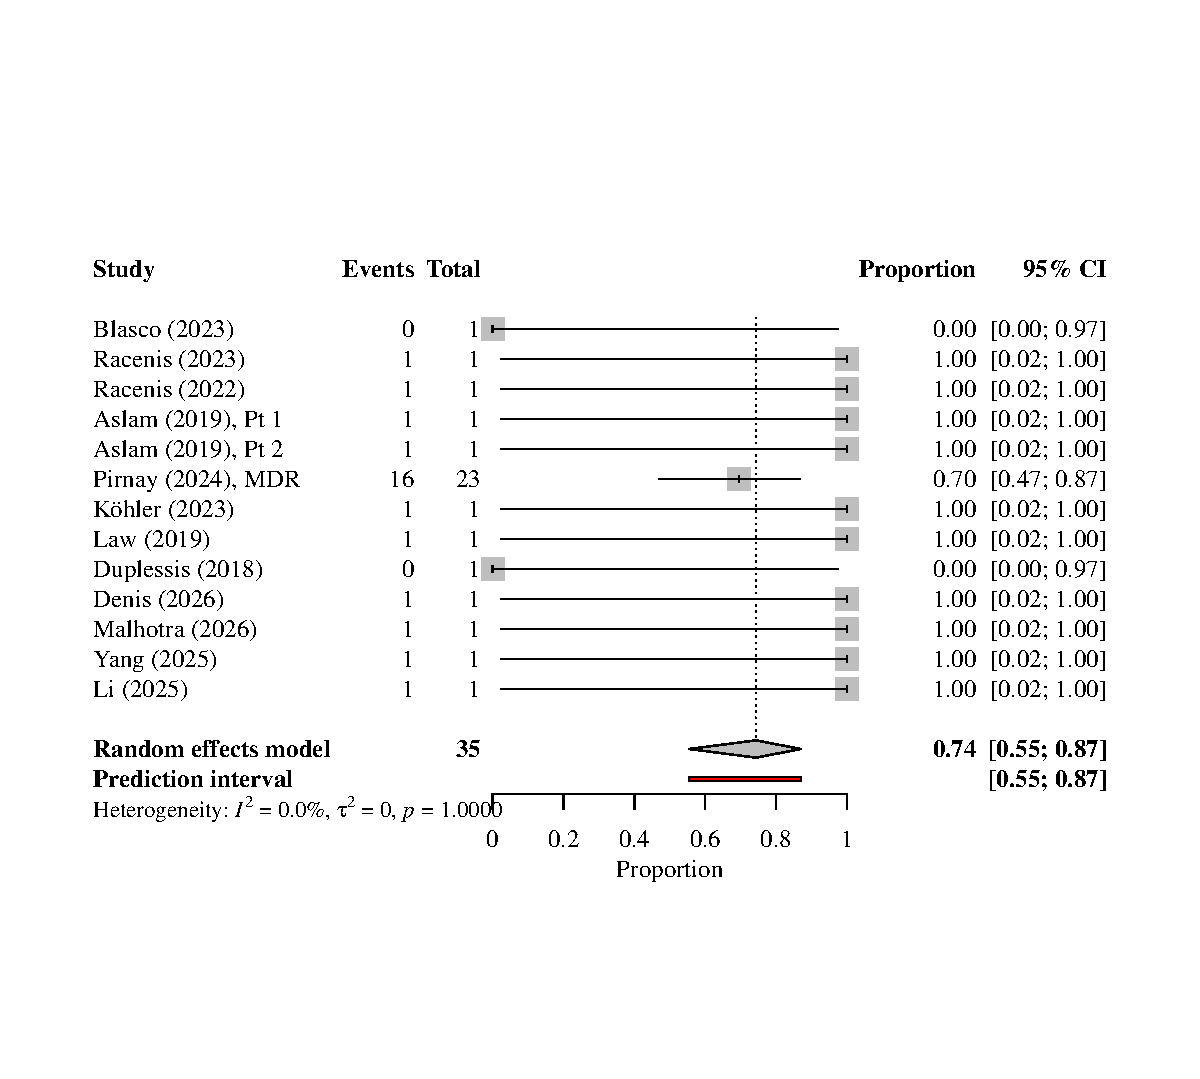
\includegraphics[width=\textwidth]{figures/phage_therapy_mdr_pseudomonas/forest_clinical_success_resistance_MDR.pdf}
\caption{MDR resistance stratum}
\label{fig:forest-success-mdr-a}
\end{subfigure}
\hfill
\begin{subfigure}{0.48\textwidth}
\centering
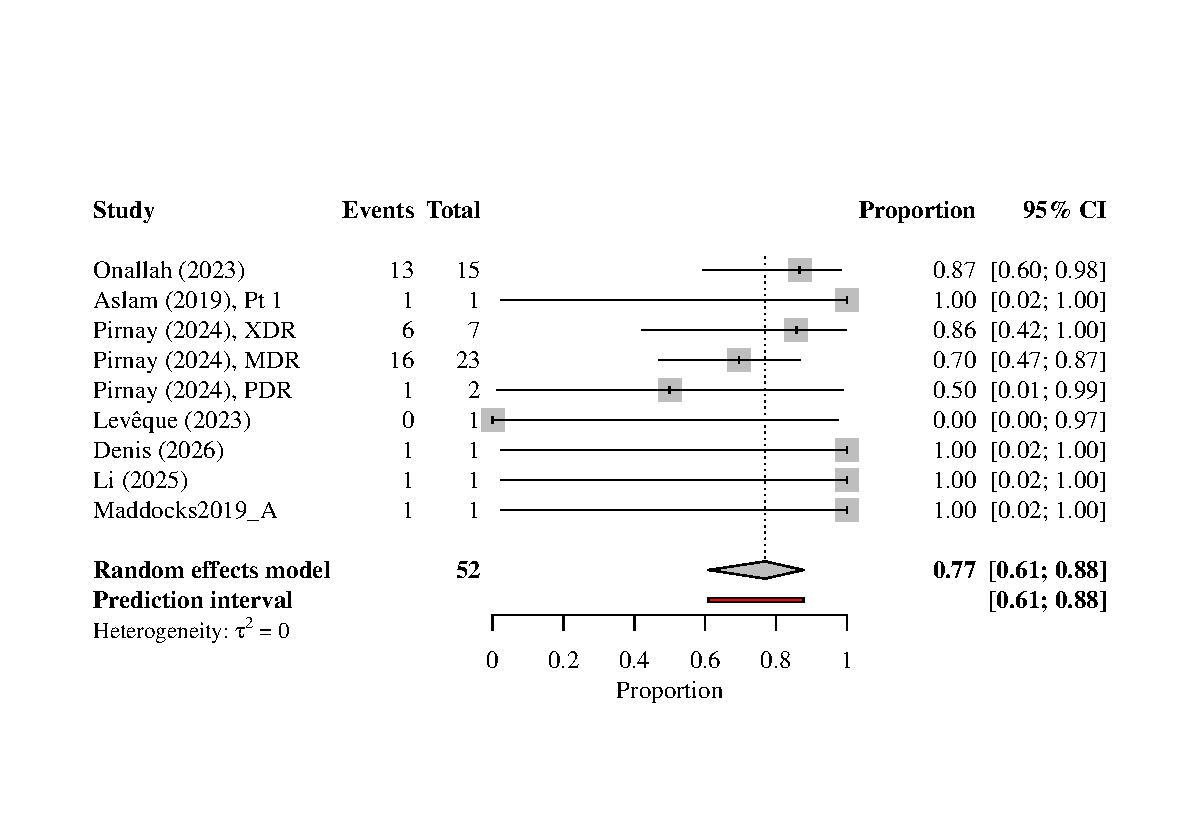
\includegraphics[width=\textwidth]{figures/phage_therapy_mdr_pseudomonas/forest_clinical_success_route_other.pdf}
\caption{Route: ``other'' (multi-route)}
\label{fig:forest-success-mdr-b}
\end{subfigure}
\caption{Forest plots: two stratified cells meeting the pooling threshold. Panel (a): clinical success among the 14 studies (37 patients) classified MDR (75.7\%, 95\% CI 57.8--87.6\%) --- a single-cohort-dominated estimate that clears the pooling threshold only under author-reported resistance labels (Section~\ref{sec:results-robustness}). Panel (b): clinical success among the 7--8 studies (38--53 patients depending on outcome) coded a multi-route or otherwise unclassifiable ("other") route (77.4\%, 95\% CI 61.9--87.8\% for clinical success). XDR, PDR, and every specific single route fell below threshold and are not plotted; see \Cref{tab:not-pooled}. Source: \texttt{scripts/R/07\_figures.R}.}
\label{fig:forest-success-mdr}
\end{figure}

Pooled safety (at least one adverse event), across 20 studies (81 patients), is 19.1\% (95\% CI 9.6--34.4\%; $\tau^2=0.085$; \Cref{fig:forest-safety-overall}). Leave-one-out does not flag the \emph{overall} safety estimate as sensitive to any single study's removal, though the MDR-specific safety estimate, the mortality-specific estimate in both the MDR and not-classifiable resistance strata, and the route-``other'' safety estimate remain sensitive to removing \citeauthor{Pirnay2024_natmicrobiol} (MDR, route-``other'') or \citeauthor{Jault2019_phagoburn} (not-classifiable mortality) specifically, collapsing to a value indistinguishable from zero on removal. The sensitivity models bracket the GLMM: Freeman-Tukey gives 7.9\% and logit-DerSimonian-Laird gives 26.8\% against the GLMM's 19.1\% (\Cref{tab:sensitivity}), and the fixed-effect model converges at 26.8\% too. Even so, the MDR- and route-specific safety/mortality estimates, and the two not-classifiable safety/mortality cells, should be read as resting heavily on one or two dominant sources, not as an even-weighted synthesis across independent studies (Section~\ref{sec:results-robustness}).

\begin{figure}[htbp]
\centering
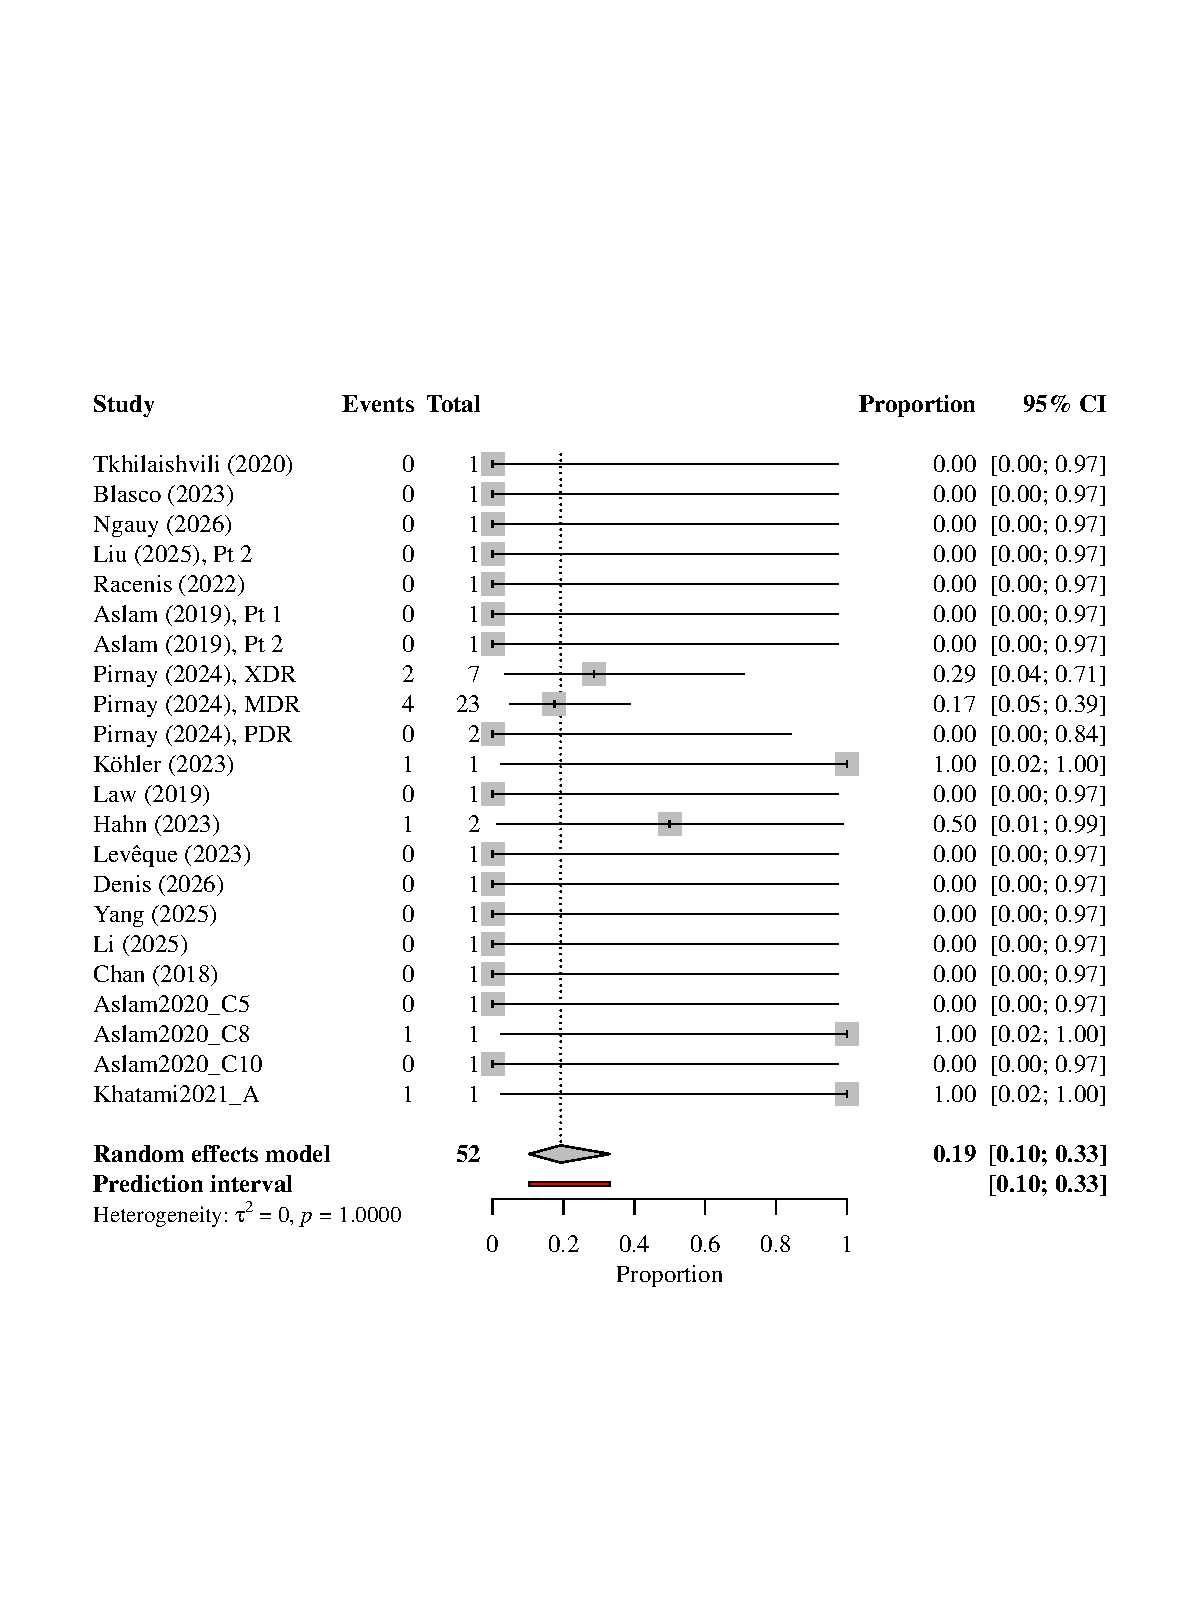
\includegraphics[width=0.8\textwidth]{figures/phage_therapy_mdr_pseudomonas/forest_safety_overall.pdf}
\caption{Forest plot: pooled safety (at least one adverse event), overall (secondary/contextual). Each row is one of the 20 studies contributing safety data (81 patients); the GLMM diamond shows 19.1\% (95\% CI 9.6--34.4\%). Leave-one-out (Section~\ref{sec:results-robustness}) no longer flags this specific estimate as sensitive to any single study's removal, though the MDR- and route-specific safety estimates remain so. Source: \texttt{scripts/R/07\_figures.R}.}
\label{fig:forest-safety-overall}
\end{figure}

\subsection{Sensitivity and Robustness Analyses}
\label{sec:results-robustness}

Transformation and model choice changes the pooled estimate by more than 5 percentage points in 12 of the 15 pooled cells; the three cells below the flag threshold are eradication overall, not-classifiable mortality, and the inhaled/nebulized safety cell (\Cref{tab:sensitivity}). Leave-one-out removal of each (arm, cell) combination shifts a pooled estimate outside its full-sample CI in exactly 4 cases: removing \citeauthor{Pirnay2024_natmicrobiol} (\citeyear{Pirnay2024_natmicrobiol}) collapses the MDR-specific safety and mortality estimates and the route-"other" safety estimate to a value numerically indistinguishable from zero, and removing \citeauthor{Jault2019_phagoburn} (\citeyear{Jault2019_phagoburn}) does the same to the not-classifiable resistance stratum's new mortality estimate. Notably, the \emph{overall} safety and mortality estimates are not shifted outside their CIs by any single-study removal. The same removals do \emph{not} overturn the clinical-success or eradication estimates in any stratum, including MDR, where Pirnay supplies the large majority of pooled patients (Section~\ref{sec:results-synthesis}) --- the instability is confined to the safety/mortality outcomes in specific strata rather than a general fragility of the MDR or not-classifiable pools. The Hartung-Knapp-Sidik-Jonkman adjustment \parencite{IntHout2014_hksj} widens the CI relative to a Wald interval in every pooled cell, confirming it as the more conservative, appropriate choice given the small number of studies per cell. Robust-variance clustering by study changes standard errors in different directions depending on the cell: eradication in the route-"other" stratum narrows substantially (naive SE 0.342 to RVE SE 0.098), while mortality in the same stratum widens (0.457 to 0.514), so the naive-independence assumption is neither confirmed nor cleanly refuted as a uniform source of bias. A classification-sensitivity check restricting to independently-verified resistance labels only (rather than the primary analysis's mix of independently-verified and author-reported labels) is materially informative for the new MDR finding: under independently-verified-only classification, the MDR cell drops to $k=3$ studies and $N=4$ patients and no longer meets the pooling threshold for any outcome --- the MDR pooled estimate reported above depends substantially on author-reported (not independently re-derived) classifications, most of them from \citeauthor{Pirnay2024_natmicrobiol}'s own per-patient antibiogram-based labels, which this review team did not re-verify against raw susceptibility data.

\begin{table}[htbp]
\centering
\scriptsize
\setlength{\tabcolsep}{3pt}
\begin{threeparttable}
\caption{Sensitivity of pooled estimates to transformation and pooling-model choice}
\label{tab:sensitivity}
\begin{tabular}{llc}
\toprule
Stratum & Model & Pooled proportion [95\% CI] \\
\midrule
Clinical success -- Overall & GLMM (primary or NA if non-convergent) & 77.6\% [65.4\%, 86.4\%] \\
Clinical success -- Overall & Freeman-Tukey double-arcsine DL & 88.4\% [76.0\%, 97.4\%] \\
Clinical success -- Overall & Logit DerSimonian-Laird & 70.9\% [63.7\%, 77.2\%] \\
Clinical success -- Overall & Fixed-effect (logit) & 70.9\% [59.6\%, 80.0\%] \\
Safety (>=1 AE) -- Overall & GLMM (primary or NA if non-convergent) & 16.0\% [7.8\%, 29.9\%] \\
Safety (>=1 AE) -- Overall & Freeman-Tukey double-arcsine DL & 5.2\% [0.5\%, 13.0\%] \\
Safety (>=1 AE) -- Overall & Logit DerSimonian-Laird & 24.8\% [20.4\%, 29.9\%] \\
Safety (>=1 AE) -- Overall & Fixed-effect (logit) & 24.8\% [15.7\%, 37.0\%] \\
Eradication -- Overall & GLMM (primary or NA if non-convergent) & 52.9\% [27.8\%, 76.6\%] \\
Eradication -- Overall & Freeman-Tukey double-arcsine DL & 50.8\% [24.5\%, 76.9\%] \\
Eradication -- Overall & Logit DerSimonian-Laird & 55.7\% [45.0\%, 65.9\%] \\
Eradication -- Overall & Fixed-effect (logit) & 55.7\% [43.1\%, 67.6\%] \\
Mortality -- Overall & GLMM (primary or NA if non-convergent) & 12.7\% [6.3\%, 24.1\%] \\
Mortality -- Overall & Freeman-Tukey double-arcsine DL & 1.8\% [0.0\%, 11.0\%] \\
Mortality -- Overall & Logit DerSimonian-Laird & 24.8\% [18.1\%, 33.0\%] \\
Mortality -- Overall & Fixed-effect (logit) & 24.8\% [15.9\%, 36.5\%] \\
Clinical success -- Resistance: MDR & GLMM (primary or NA if non-convergent) & 75.7\% [57.8\%, 87.6\%] \\
Clinical success -- Resistance: MDR & Freeman-Tukey double-arcsine DL & 86.7\% [70.4\%, 98.0\%] \\
Clinical success -- Resistance: MDR & Logit DerSimonian-Laird & 69.1\% [61.9\%, 75.4\%] \\
Clinical success -- Resistance: MDR & Fixed-effect (logit) & 69.1\% [54.7\%, 80.6\%] \\
Safety (>=1 AE) -- Resistance: MDR & GLMM (primary or NA if non-convergent) & 16.7\% [7.0\%, 34.6\%] \\
Safety (>=1 AE) -- Resistance: MDR & Freeman-Tukey double-arcsine DL & 5.1\% [0.0\%, 16.9\%] \\
Safety (>=1 AE) -- Resistance: MDR & Logit DerSimonian-Laird & 24.7\% [18.1\%, 32.7\%] \\
Safety (>=1 AE) -- Resistance: MDR & Fixed-effect (logit) & 24.7\% [14.0\%, 39.6\%] \\
Eradication -- Resistance: MDR & GLMM (primary or NA if non-convergent) & 58.1\% [12.5\%, 93.1\%] \\
Eradication -- Resistance: MDR & Freeman-Tukey double-arcsine DL & 50.7\% [15.3\%, 85.8\%] \\
Eradication -- Resistance: MDR & Logit DerSimonian-Laird & 55.5\% [41.9\%, 68.3\%] \\
Eradication -- Resistance: MDR & Fixed-effect (logit) & 55.5\% [40.7\%, 69.3\%] \\
Mortality -- Resistance: MDR & GLMM (primary or NA if non-convergent) & 6.5\% [1.9\%, 19.8\%] \\
Mortality -- Resistance: MDR & Freeman-Tukey double-arcsine DL & 0.0\% [0.0\%, 2.2\%] \\
Mortality -- Resistance: MDR & Logit DerSimonian-Laird & 19.7\% [13.8\%, 27.4\%] \\
Mortality -- Resistance: MDR & Fixed-effect (logit) & 19.7\% [10.9\%, 33.0\%] \\
Clinical success -- Route: other & GLMM (primary or NA if non-convergent) & 77.4\% [61.9\%, 87.8\%] \\
Clinical success -- Route: other & Freeman-Tukey double-arcsine DL & 87.4\% [72.6\%, 97.9\%] \\
Clinical success -- Route: other & Logit DerSimonian-Laird & 73.6\% [63.2\%, 81.8\%] \\
Clinical success -- Route: other & Fixed-effect (logit) & 73.6\% [60.1\%, 83.7\%] \\
Safety (>=1 AE) -- Route: other & GLMM (primary or NA if non-convergent) & 15.8\% [6.3\%, 34.3\%] \\
Safety (>=1 AE) -- Route: other & Freeman-Tukey double-arcsine DL & 4.8\% [0.8\%, 10.8\%] \\
Safety (>=1 AE) -- Route: other & Logit DerSimonian-Laird & 21.5\% [17.9\%, 25.5\%] \\
Safety (>=1 AE) -- Route: other & Fixed-effect (logit) & 21.5\% [11.7\%, 36.0\%] \\
Eradication -- Route: other & GLMM (primary or NA if non-convergent) & 63.2\% [44.1\%, 78.8\%] \\
Eradication -- Route: other & Freeman-Tukey double-arcsine DL & 68.6\% [46.3\%, 88.1\%] \\
Eradication -- Route: other & Logit DerSimonian-Laird & 61.6\% [50.7\%, 71.4\%] \\
Eradication -- Route: other & Fixed-effect (logit) & 61.6\% [46.0\%, 75.1\%] \\
Mortality -- Route: other & GLMM (primary or NA if non-convergent) & 16.0\% [3.6\%, 48.9\%] \\
Mortality -- Route: other & Freeman-Tukey double-arcsine DL & 5.9\% [0.0\%, 31.2\%] \\
Mortality -- Route: other & Logit DerSimonian-Laird & 23.2\% [11.3\%, 41.6\%] \\
Mortality -- Route: other & Fixed-effect (logit) & 23.2\% [11.9\%, 40.3\%] \\
\bottomrule
\end{tabular}

\begin{tablenotes}
\small
\item \textit{Notes:} All 15 cells meeting the pre-specified pooling threshold (\Cref{tab:pooled-estimates}), compared across the primary random-effects binomial-normal GLMM (logit link), the Freeman-Tukey double-arcsine transformation with DerSimonian-Laird pooling \parencite{FreemanTukey1950,DerSimonianLaird1986}, a logit transformation with DerSimonian-Laird pooling, and a fixed-effect (logit) model. Divergence exceeding 5 percentage points between GLMM and the sensitivity models is reported as a finding in the text (Section~\ref{sec:results-robustness}), not a footnote. Source: \texttt{scripts/R/05\_robustness.R}, \texttt{08\_tables.R}.
\end{tablenotes}
\end{threeparttable}
\end{table}

An appendix-only relaxation of the threshold to at least 2 studies and 10 patients (\Cref{tab:threshold-relaxation}) newly qualifies several cells beyond the primary set --- clinical success in the not-classifiable resistance stratum ($k=2$, $N=16$), safety and mortality in the topical/local route ($k=5$, $N=18$ each, the topical/local arms enlarged by the newly added \citeauthor{Chan2018_omko1_emph} case), and all four XDR outcome cells ($k=4$, $N=10$ each, having just reached the ten-patient relaxed floor as the corpus grew) --- while PDR and intravenous remain below even the relaxed threshold. (Safety in the inhaled/nebulized route, previously below threshold, now clears the \emph{primary} threshold and appears in \Cref{tab:pooled-estimates} rather than here.) These estimates are reported only to show that the primary threshold is itself consequential; none is promoted to a primary result. A study-design-stratified comparison (RCT/cohort vs.\ case report/series) found no significant subgroup difference for clinical success (Q-between $p=0.285$), and a collapsed systemic-versus-local (2-category) route taxonomy likewise found none ($p=0.53$). A geographic-concentration exclusion of the Belgium and Israel cohorts --- which together supply the two largest sources in the corpus, \citeauthor{Pirnay2024_natmicrobiol} and \citeauthor{Onallah2023_med} --- now leaves all four overall outcomes above the pooling threshold: clinical success (0.776, essentially unchanged at 0.800 once excluded), safety (0.191 falling to 0.140), eradication (0.551 rising to 0.685), and mortality (0.105 falling to 0.037). That the enlarged corpus retains all four overall estimates even without its two dominant cohorts is a robustness improvement over earlier versions of this review, in which removing them pushed clinical success (and, earlier still, eradication) below the pooling threshold. A Liu et al.\ reuse-tier transparency check confirms every one of the 30 pooling-eligible rows is coded \texttt{data\_provenance == independently-extracted} (Section~\ref{sec:methods-extraction}); no row uses Tier-3 (directly adopted) data, so the independently-extracted-only and all-rows pooled estimates are identical by construction, reported as a transparency confirmation rather than a contrast.

\begin{table}[htbp]
\centering
\scriptsize
\setlength{\tabcolsep}{3pt}
\begin{threeparttable}
\caption{Appendix: effect of relaxing the pooling threshold to $k \geq 2$ studies and $N \geq 10$ patients}
\label{tab:threshold-relaxation}
\begin{tabular}{lllccl}
\toprule
Outcome -- Stratum & Primary$^a$ & Relaxed$^b$ & $k$ (relaxed) & $N$ (relaxed) & Flag \\
\midrule
Clinical success -- Overall & POOLED & POOLED & 23 & 71 &  \\
Safety (>=1 AE) -- Overall & POOLED & POOLED & 18 & 53 &  \\
Eradication -- Overall & POOLED & POOLED & 20 & 60 &  \\
Mortality -- Overall & POOLED & POOLED & 24 & 67 &  \\
Clinical success -- Resistance: MDR & POOLED & POOLED & 15 & 38 &  \\
Clinical success -- Resistance: NC & NOT\_POOLED & POOLED & 4 & 19 & NEW (relaxed) \\
Clinical success -- Resistance: PDR & NOT\_POOLED & NOT\_POOLED & 3 & 4 &  \\
Clinical success -- Resistance: XDR & NOT\_POOLED & POOLED & 4 & 10 & NEW (relaxed) \\
Safety (>=1 AE) -- Resistance: MDR & POOLED & POOLED & 13 & 37 &  \\
Safety (>=1 AE) -- Resistance: NC & NOT\_POOLED & NOT\_POOLED & 1 & 2 &  \\
Safety (>=1 AE) -- Resistance: PDR & NOT\_POOLED & NOT\_POOLED & 3 & 4 &  \\
Safety (>=1 AE) -- Resistance: XDR & NOT\_POOLED & POOLED & 4 & 10 & NEW (relaxed) \\
Eradication -- Resistance: MDR & POOLED & POOLED & 14 & 43 &  \\
Eradication -- Resistance: NC & NOT\_POOLED & NOT\_POOLED & 1 & 1 &  \\
Eradication -- Resistance: PDR & NOT\_POOLED & NOT\_POOLED & 4 & 6 &  \\
Eradication -- Resistance: XDR & NOT\_POOLED & POOLED & 4 & 10 & NEW (relaxed) \\
Mortality -- Resistance: MDR & POOLED & POOLED & 17 & 47 &  \\
Mortality -- Resistance: NC & NOT\_POOLED & NOT\_POOLED & 3 & 4 &  \\
Mortality -- Resistance: PDR & NOT\_POOLED & NOT\_POOLED & 4 & 6 &  \\
Mortality -- Resistance: XDR & NOT\_POOLED & POOLED & 4 & 10 & NEW (relaxed) \\
Clinical success -- Route: inhaled/nebulized & NOT\_POOLED & NOT\_POOLED & 2 & 2 &  \\
Clinical success -- Route: IV & NOT\_POOLED & NOT\_POOLED & 6 & 8 &  \\
Clinical success -- Route: other & POOLED & POOLED & 9 & 54 &  \\
Clinical success -- Route: topical/local & NOT\_POOLED & NOT\_POOLED & 5 & 5 &  \\
Safety (>=1 AE) -- Route: inhaled/nebulized & NOT\_POOLED & NOT\_POOLED & 3 & 4 &  \\
Safety (>=1 AE) -- Route: IV & NOT\_POOLED & NOT\_POOLED & 5 & 7 &  \\
Safety (>=1 AE) -- Route: other & POOLED & POOLED & 7 & 38 &  \\
Safety (>=1 AE) -- Route: topical/local & NOT\_POOLED & NOT\_POOLED & 4 & 4 &  \\
Eradication -- Route: inhaled/nebulized & NOT\_POOLED & NOT\_POOLED & 3 & 11 &  \\
Eradication -- Route: IV & NOT\_POOLED & NOT\_POOLED & 5 & 5 &  \\
Eradication -- Route: other & POOLED & POOLED & 8 & 39 &  \\
Eradication -- Route: topical/local & NOT\_POOLED & NOT\_POOLED & 4 & 4 &  \\
Mortality -- Route: inhaled/nebulized & NOT\_POOLED & NOT\_POOLED & 4 & 13 &  \\
Mortality -- Route: IV & NOT\_POOLED & NOT\_POOLED & 6 & 8 &  \\
Mortality -- Route: other & POOLED & POOLED & 8 & 39 &  \\
Mortality -- Route: topical/local & NOT\_POOLED & NOT\_POOLED & 5 & 5 &  \\
\bottomrule
\end{tabular}

\begin{tablenotes}
\small
\item \textit{Notes:} Supplementary sensitivity check, not a primary result. Compares each cell's pooling status under the primary threshold ($k \geq 3$, $N \geq 20$) against a relaxed threshold ($k \geq 2$, $N \geq 10$). Cells flagged "NEW (relaxed)" are reported for transparency about threshold sensitivity and are not promoted to \Cref{tab:pooled-estimates} or cited elsewhere as primary findings. Source: \texttt{scripts/R/05\_robustness.R}, \texttt{08\_tables.R}.
\item[a] Pooling status under the primary threshold ($k \geq 3$ studies, $N \geq 20$ patients).
\item[b] Pooling status under the relaxed threshold ($k \geq 2$ studies, $N \geq 10$ patients).
\end{tablenotes}
\end{threeparttable}
\end{table}

\subsection{Falsification and Negative-Control Checks}
\label{sec:results-falsification}

Most of the six pre-specified falsification checks are null or pass as expected. A meta-regression of transformed clinical success on publication year found no secular trend (logit-scale coefficient $0.030$, $p=0.81$), arguing against a reporting-drift explanation. A cross-tabulation of route by resistance class by geographic source found no route confined to a single region, arguing against a route effect that is actually a single-center signature. The one check that does not fully pass is the journal-tier comparison: high-tier journals report a higher pooled clinical-success proportion (79.6\%, 8 studies) than mid-tier journals (69.2\%, 12 studies), a roughly 10-percentage-point gap. With only two tiers and small per-tier counts this is not formally tested and should not be over-read, but the gradient is in the direction a selective-reporting or editorial-selection effect would produce, and is reported here as a mild caution rather than a clean pass. The length-of-hospitalization comparison remains not applicable: only 1 of the 30 arms reports a value, too sparse for even a qualitative check.

Peters' regression test for funnel-plot asymmetry, applied to the four outcome-overall cells with at least 10 studies as pre-specified, is non-significant for every tested outcome: clinical success ($p=0.66$), safety ($p=0.38$), eradication ($p=0.82$), and mortality ($p=0.24$; \Cref{fig:funnel-eyeball}). These four outcome-overall cells are the only ones that can support the test; the MDR-specific and other resistance-stratified cells have too few studies for Peters' regression and return no estimate (NA), so no small-study test is reported for them. Peters' test replaces the Egger's linear regression an earlier version of this review applied here, and the substitution reverses the earlier apparent finding. Egger's test is invalid for a meta-analysis of proportions: the standard error is a deterministic function of the proportion and manufactures funnel asymmetry near the 0/1 boundary. The earlier ``mortality signal'' ($p=0.02$ under Egger's) was an artifact of exactly that failure mode --- a mortality funnel dominated by single-patient arms at 0\% and two at 100\% --- not genuine small-study bias; under the appropriate Peters' test mortality asymmetry is not significant ($p=0.24$), and no outcome is. We read this as reassurance, but weak reassurance: non-significance in a corpus of 30 study-arms that remains small and, as Section~\ref{sec:results-robustness}'s leave-one-out and classification-sensitivity checks show, dependent on one or two dominant sources in several strata, is the absence of a detectable small-study effect under a test the data can properly support, not a clean acquittal.

\begin{figure}[htbp]
\centering
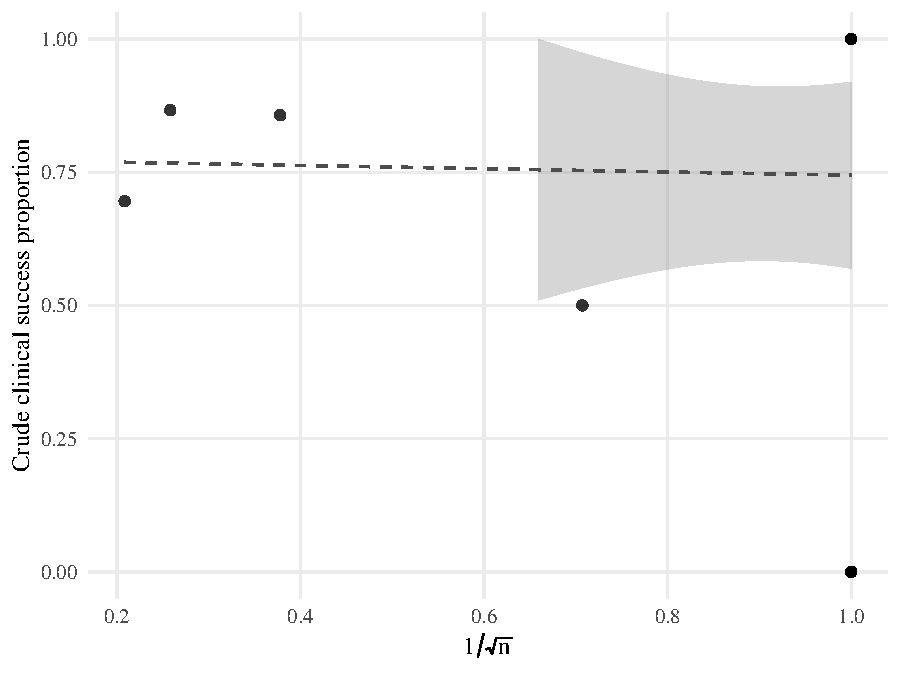
\includegraphics[width=0.8\textwidth]{figures/phage_therapy_mdr_pseudomonas/small_study_eyeball.pdf}
\caption{Small-study effects: crude proportion versus $1/\sqrt{n}$. Each point is one pooling-eligible study-arm; the $x$-axis is the inverse square root of arm sample size (a proxy for precision), the $y$-axis is the arm's crude, untransformed outcome proportion. A visual complement to the formal Peters' regression test (clinical success $p=0.66$, safety $p=0.38$, eradication $p=0.82$, mortality $p=0.24$; none significant), applied to the four outcome-overall cells with at least 10 studies per the pre-specified threshold; the resistance-stratified cells have too few studies to support the test. Source: \texttt{scripts/R/06\_falsification.R}, \texttt{07\_figures.R}.}
\label{fig:funnel-eyeball}
\end{figure}

\subsection{Certainty of Evidence (GRADE)}
\label{sec:results-grade}

Certainty of evidence was rated for all 15 pooled cells (Section~\ref{sec:methods-rob}). \textbf{Every cell is rated Very low.} That uniform verdict is not a formality: it follows from each cell starting at Low certainty --- the GRADE default for uncontrolled observational evidence, which is what a single-arm proportion drawn from compassionate-use case reports is --- and then being rated down at least twice more, so that all cells reach GRADE's floor. The practical implication is direct: none of the proportions reported above should be used to inform a treatment decision, and the review's contribution lies in mapping where evidence is absent rather than in the point estimates themselves.

The domain profile in \Cref{tab:grade} nonetheless discriminates sharply among cells, and that profile is more informative than the floored rating. Three cells carry the minimum burden of three downgrades --- overall safety, overall mortality, and the route-``other'' safety estimate --- each rated down once for risk of bias, once for the salvage-population indirectness common to every cell, and once for suspected publication bias, but not for inconsistency or imprecision. At the other extreme, MDR eradication accumulates seven downgrades' worth of problems (risk of bias, very serious inconsistency with a prediction interval spanning almost the entire 0--100\% range, indirectness, very serious imprecision, and publication bias), as do the not-classifiable safety cell and the inhaled/nebulized safety cell. The four clinical-success cells each take a second indirectness downgrade because success is defined by each primary study on its own terms across non-comparable infection syndromes (Section~\ref{sec:methods-eligibility}), so the pooled construct is not a single clinical outcome. Two structural downgrades apply to every cell without exception --- the compassionate-use salvage population, and publication bias --- and neither can be remedied by adding more case reports of the same kind.

\begin{table}[htbp]
\centering
\scriptsize
\setlength{\tabcolsep}{3pt}
\begin{threeparttable}
\caption{GRADE certainty of evidence for the 15 pooled outcome-stratum cells}
\label{tab:grade}
\begin{tabular}{lccclccccc l}
\toprule
Outcome -- Stratum & $k$ & Arms & $N$ & Pooled proportion [95\% CI] & RoB & Incons. & Indir. & Imprec. & Pub.\ bias & Certainty \\
\midrule
Clinical success -- Overall & 23 & 28 & 71 & 76.1\% [64.2, 84.9] & $-$1 & -- & $-$2 & -- & $-$1 & Very low \\
Safety (>=1 AE) -- Overall & 18 & 23 & 53 & 17.0\% [8.7, 30.4] & $-$1 & -- & $-$1 & -- & $-$1 & Very low \\
Eradication -- Overall & 20 & 24 & 60 & 55.1\% [29.4, 78.4] & $-$1 & $-$2 & $-$1 & $-$1 & $-$1 & Very low \\
Mortality -- Overall & 24 & 30 & 67 & 11.9\% [5.9, 22.7] & $-$1 & -- & $-$1 & -- & $-$1 & Very low \\
Clinical success -- Resistance: MDR & 15 & 16 & 38 & 73.7\% [56.1, 86.0] & $-$1 & -- & $-$2 & -- & $-$1 & Very low \\
Safety (>=1 AE) -- Resistance: MDR & 13 & 14 & 37 & 16.2\% [6.9, 33.7] & $-$1 & -- & $-$1 & -- & $-$1 & Very low \\
Eradication -- Resistance: MDR & 14 & 15 & 43 & 58.1\% [12.5, 93.1] & $-$1 & $-$2 & $-$1 & $-$2 & $-$1 & Very low \\
Mortality -- Resistance: MDR & 17 & 18 & 47 & 6.4\% [1.9, 19.4] & $-$1 & -- & $-$1 & -- & $-$1 & Very low \\
Clinical success -- Route: other & 9 & 11 & 54 & 77.8\% [62.8, 87.9] & $-$1 & -- & $-$2 & -- & $-$1 & Very low \\
Safety (>=1 AE) -- Route: other & 7 & 9 & 38 & 15.8\% [6.3, 34.3] & $-$1 & -- & $-$1 & -- & $-$1 & Very low \\
Eradication -- Route: other & 8 & 10 & 39 & 64.1\% [45.6, 79.2] & $-$1 & -- & $-$1 & $-$1 & $-$1 & Very low \\
Mortality -- Route: other & 8 & 10 & 39 & 15.4\% [6.2, 33.2] & $-$1 & -- & $-$1 & -- & $-$1 & Very low \\
\bottomrule
\end{tabular}

\begin{tablenotes}
\small
\item \textit{Notes:} All bodies of evidence start at \emph{Low} certainty (GRADE's default for observational evidence; every cell is an uncontrolled single-arm proportion) and are rated down across five domains. Domain columns give the number of certainty levels deducted; "--" denotes no downgrade. Certainty cannot fall below \emph{Very low} (GRADE's floor), so cells differing widely in their domain burden share the same final rating --- the profile, not the rating alone, carries the information. Rating rules are pre-specified and applied to each cell's own data rather than judged case by case: risk of bias from the share of patients contributed by single-patient case reports and the presence of the one High-risk-of-bias trial; inconsistency from the 95\% prediction-interval width; indirectness from the compassionate-use salvage population, with a second level for clinical success (defined per study across non-comparable syndromes); imprecision from the 95\% CI width; publication bias strongly suspected throughout (favourable-outcome reporting is intrinsic to a compassionate-use case-report literature and Peters' test cannot exclude it at this corpus size). No upgrade criterion applied. Source: \texttt{scripts/R/10\_grade.R}.
\end{tablenotes}
\end{threeparttable}
\end{table}
